\documentclass[tikz,border=3mm]{standalone}
\usepackage[T1]{fontenc}
\usetikzlibrary{arrows.meta,positioning}
\begin{document}
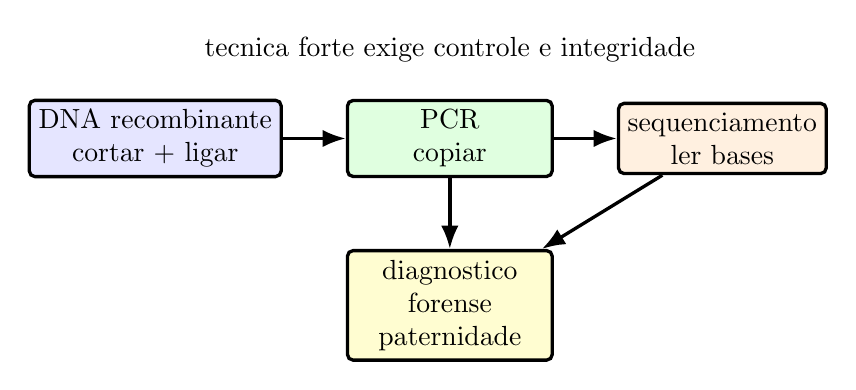
\begin{tikzpicture}[>=Latex,node distance=0.8cm]
  \tikzstyle{box}=[draw,rounded corners=2pt,very thick,align=center,minimum width=2.6cm,minimum height=0.75cm]
  \node[box,fill=blue!10] (rec) {DNA recombinante\\cortar + ligar};
  \node[box,fill=green!12,right=0.8cm of rec] (pcr) {PCR\\copiar};
  \node[box,fill=orange!12,right=0.8cm of pcr] (seq) {sequenciamento\\ler bases};
  \node[box,fill=yellow!18,below=0.9cm of pcr] (uso) {diagnostico\\forense\\paternidade};
  \draw[very thick,->] (rec) -- (pcr);
  \draw[very thick,->] (pcr) -- (seq);
  \draw[very thick,->] (pcr) -- (uso);
  \draw[very thick,->] (seq) -- (uso);
  \node[align=center,above=0.35cm of pcr] {tecnica forte exige controle e integridade};
\end{tikzpicture}
\end{document}
